\documentclass[conference]{IEEEtran}
\IEEEoverridecommandlockouts
\usepackage{cite}
\usepackage{amsmath,amssymb,amsfonts}
\usepackage{algorithmic}
\usepackage{graphicx}
\usepackage{textcomp}
\usepackage{xcolor}
\usepackage{booktabs}
\usepackage{url}
\usepackage[utf8]{inputenc}
\usepackage[T5,T1]{fontenc}
\def\BibTeX{{\rm B\kern-.05em{\sc i\kern-.025em b}\kern-.08em
    T\kern-.1667em\lower.7ex\hbox{E}\kern-.125emX}}

\begin{document}

\title{Eco-Conscious AI-Powered Multimodal Product Recommendation System for Vietnamese E-Commerce}

\author{\IEEEauthorblockN{{\fontencoding{T5}\selectfont Đạt Nguyễn, Đức Đặng, Quyên Huỳnh, Hà Nguyễn}, Baptiste Monsterleet, and Thomas Portelette}
\IEEEauthorblockA{International Institute of Technology DNIIT, The University of Danang, Vietnam}}

\maketitle

\begin{abstract}
The rapid growth of Vietnam's e-commerce sector has given consumers broad access to consumer electronics and home appliances, yet significant obstacles persist. Product data is fragmented across competing platforms, making price and warranty comparisons tedious. Furthermore, retailers provide virtually no transparency regarding the environmental impact of the products they sell. This paper presents \textit{Smart Product Finder}, an AI-powered multimodal search engine tailored for the Vietnamese market. The system employs daily-scheduled Scrapy web scrapers orchestrated by Apache Airflow to aggregate product data from five major Vietnamese retailers through an Apache Kafka event-streaming pipeline. Multimodal embeddings are generated using OpenCLIP (ViT-B-32) and indexed in dual FAISS vector stores for fast text and image retrieval. A three-stage recommendation pipeline first retrieves the top 50 semantically similar candidates, re-ranks them with a CatBoost learning-to-rank model evaluated on seven criteria, and finally fuses the relevance ranking with carbon footprint estimates via weighted Reciprocal Rank Fusion (RRF). To address the absence of official Environmental Product Declarations (EPDs), a local Large Language Model (Qwen~3.5 0.8B, served by Ollama) generates cradle-to-grave CO\textsubscript{2} estimates using either an anchored or unanchored prompting strategy depending on reference data availability, validated against 41 category-specific plausibility bounds. Leave-one-out validation on a 30-product sample shows strong ordinal consistency (Spearman~$\rho = 0.923$), though absolute accuracy remains a challenge (MAE~$= 77.2$\,kg) particularly for broad product categories. The deployment highlights practical challenges including processing latency, model limitations, and data acquisition constraints imposed by budget restrictions.
\end{abstract}

\begin{IEEEkeywords}
E-commerce, Recommender Systems, Multimodal Retrieval, Reciprocal Rank Fusion, Carbon Footprint Estimation, CatBoost, Learning to Rank, Local LLM
\end{IEEEkeywords}

% ================================================================
\section{Introduction}
% ================================================================

Vietnam's digital economy has undergone rapid transformation, with e-commerce revenues growing steadily year over year. Despite this expansion, consumers face a significant cognitive burden when shopping for electronics and home appliances online. Comparing prices, warranties, return policies, and seller reliability across major Vietnamese retail platforms requires tedious manual navigation through fragmented and cluttered user interfaces. Finding the genuinely ``best offer'' for a given product remains an inefficient process.

Compounding this issue is a distinct lack of ecological transparency. Official Environmental Product Declarations (EPDs) and Life Cycle Assessment (LCA) data are rarely available for consumer products in the Vietnamese market, making it virtually impossible for environmentally conscious shoppers to factor carbon footprint into their purchasing decisions. Recent research has demonstrated that post-hoc carbon-aware re-ranking can achieve substantial environmental improvements---reducing recommended product carbon footprints by 70--86\%---with only minimal losses in recommendation relevance~\cite{carbon_reranking, ecommerce_carbon}.

To address these dual challenges of market fragmentation and ecological opacity, we developed \textit{Smart Product Finder}, an intelligent multimodal search engine that aggregates product data across platforms, optimizes recommendations through multi-criteria ranking, and estimates the environmental impact of products. The principal contributions of this work are as follows:

\begin{enumerate}
    \item A complete microservices-based platform that aggregates product data from five major Vietnamese electronics and appliance retailers through a daily Airflow-orchestrated, Kafka-mediated data pipeline.
    \item A multimodal search system supporting both text and image queries, powered by OpenCLIP embeddings and dual FAISS vector indexes.
    \item A hybrid three-stage ranking pipeline combining FAISS retrieval, CatBoost learning-to-rank, and weighted Reciprocal Rank Fusion (RRF) with carbon footprint estimates.
    \item A two-stage local LLM pipeline for estimating cradle-to-grave CO\textsubscript{2} emissions using a lightweight quantized model (Qwen~3.5 0.8B), anchored by a curated reference dataset of known carbon footprints.
\end{enumerate}

% ================================================================
\section{Related Work}
% ================================================================

\subsection{E-Commerce Recommendation and Price Comparison}

Recent advances in e-commerce recommendation have explored diverse methodological avenues. Deep Reinforcement Learning (DRL) combined with TensorFlow Recommenders (TFRS) has been shown to improve recommendation accuracy by 15--25\% over static models~\cite{paper1}. Cost-effective architectures utilizing TF-IDF vectorization and cosine similarity have been proposed to empower small and medium enterprises (SMEs) against larger marketplaces~\cite{paper2}. AI-powered price comparison systems have employed predictive models including Random Forest and LSSVM to forecast price trends across e-commerce and food delivery platforms~\cite{paper3}. Multi-agent systems integrating NLP chatbots have demonstrated the potential for automated shopping optimization across multiple vendors~\cite{paper4}.

\subsection{Multimodal Retrieval}

Beyond traditional keyword matching, modern retrieval systems adopt multimodal approaches. Zhang et al.~\cite{paper5} proposed a multi-modal retrieval architecture fusing BLIP, CLIP, and CLIP Interrogator to bridge the gap between natural language queries and visual product representations, demonstrating superior image-text alignment over keyword-based search. OpenCLIP~\cite{openclip} provides open-source contrastive language--image models trained on large-scale datasets, enabling high-quality zero-shot embeddings for both text and images.

\subsection{Carbon-Aware Recommendation}

The intersection of sustainability and recommender systems is an emerging research area. Vestrum et al.~\cite{carbon_reranking} introduced a retrieval-augmented Product Carbon Footprint (PCF) estimation pipeline using few-shot LLM prompting anchored by the Carbon Catalogue, demonstrating that under a modest 5\% NDCG budget loss, carbon footprint reductions of 70--86\% are achievable through post-hoc re-ranking. Spillo et al.~\cite{ecommerce_carbon} presented the Eco-Amazon dataset, enriching e-commerce catalogs with LLM-estimated carbon footprints and demonstrating high ordinal ranking consistency (Spearman $\rho > 0.9$) even when absolute gram-level precision varies. Xu et al.~\cite{carbon_estimation} proposed a Progressive Layered Extraction (PLE) multi-task learning model for carbon estimation in electromechanical manufacturing, achieving $R^2 \approx 0.94$.

Our work builds upon these multimodal and sustainability-aware concepts, introducing a practical ranking fusion strategy tailored to the data-scarce Vietnamese market, utilizing a lightweight local LLM for carbon estimation to avoid dependency on cloud-based APIs.

% ================================================================
\section{System Architecture}
% ================================================================

\subsection{Overview}

The Smart Product Finder platform is built on a fully containerized microservices architecture, orchestrated through Docker Compose. Fig.~\ref{fig:architecture} illustrates the high-level system design, comprising five principal layers: data collection, event streaming, data processing, storage, and presentation. This decoupled design ensures that resource-intensive background operations (scraping, embedding generation, carbon estimation) do not degrade the responsiveness of user-facing search queries.

\begin{figure}[htbp]
\centerline{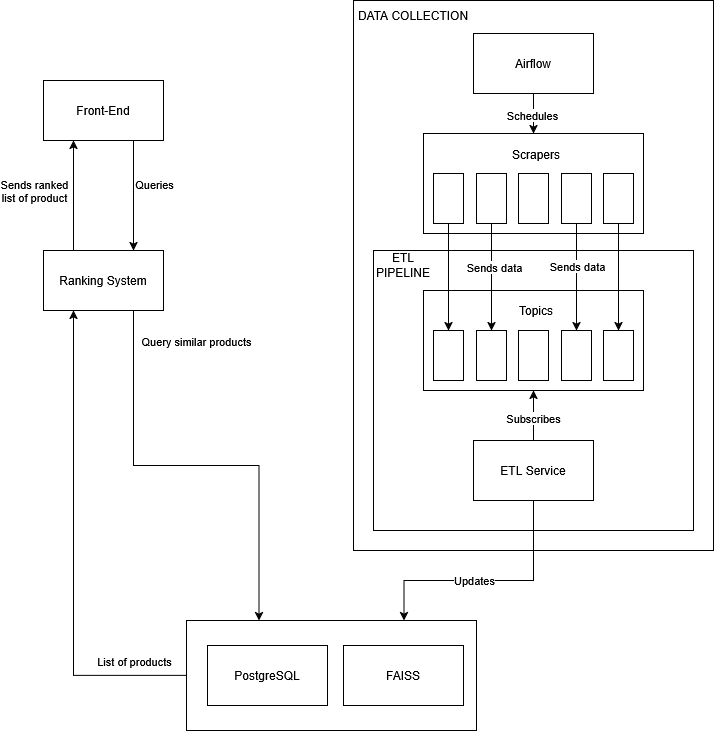
\includegraphics[width=\columnwidth]{fig_architecture}}
\caption{System architecture overview. Data collection (right) is orchestrated by Apache Airflow, which schedules Scrapy spiders to extract product data from five Vietnamese retailers. Raw data flows through platform-specific Apache Kafka topics to an ETL service, which generates OpenCLIP embeddings and persists structured metadata to PostgreSQL and vector embeddings to dual FAISS indexes. The Ranking System (left) serves user queries by retrieving candidates from FAISS, re-ranking with CatBoost, and fusing with carbon estimates via RRF.}
\label{fig:architecture}
\end{figure}

\subsection{Data Collection Pipeline}

Product data is collected from five major Vietnamese electronics and appliance retailers: CellphoneS, Phong V\~{u}, FPT Shop, Th\'{e} Gi\'{o}i Di \DJ\d{o}ng (TGDD), and \DJ i\d{e}n M\'ay Xanh (DMX). Custom Scrapy web spiders are implemented for each platform, scheduled to execute daily via Apache Airflow DAGs. This daily batch approach was chosen because product catalogs update infrequently, and high-frequency scraping would exhaust server resources without adding meaningful value.

Several platforms employ anti-bot protections. For Cloudflare-protected sites, we integrate a local FlareSolverr proxy container that automatically solves challenge tokens and maintains valid session cookies, avoiding the cost of commercial proxy services. Major marketplace platforms such as Shopee and Lazada were excluded due to aggressive anti-bot measures requiring residential proxy rotation, which was cost-prohibitive given the project's budget constraints.

Each spider publishes raw product data to platform-specific Apache Kafka topics, providing asynchronous decoupling between the scraping and processing stages. An ETL worker service subscribes to these topics, validates and normalizes the incoming data, requests multimodal embeddings from the OpenCLIP service, estimates carbon footprints via the local LLM, and persists the results to the storage layer.

\subsection{Embedding Generation and Storage}

The ETL worker generates dense multimodal vector representations for each product using OpenCLIP~\cite{openclip} with the ViT-B-32 architecture, pretrained on the LAION-2B dataset. Both textual embeddings (derived from product names and descriptions) and visual embeddings (derived from product images) are computed. These embeddings are indexed in two separate FAISS~\cite{faiss} vector stores---one for text and one for images---using an inner-product similarity index (\texttt{IndexFlatIP}). Structured product metadata (prices, ratings, seller information, return policies, warranties) is stored in a PostgreSQL relational database.

% ================================================================
\section{Methodology}
% ================================================================

\subsection{Multimodal Search and Retrieval}

The system supports three query modalities: text-only, image-only, and combined text-and-image queries. Fig.~\ref{fig:pipeline} illustrates the complete retrieval and ranking pipeline.

\begin{figure}[htbp]
\centerline{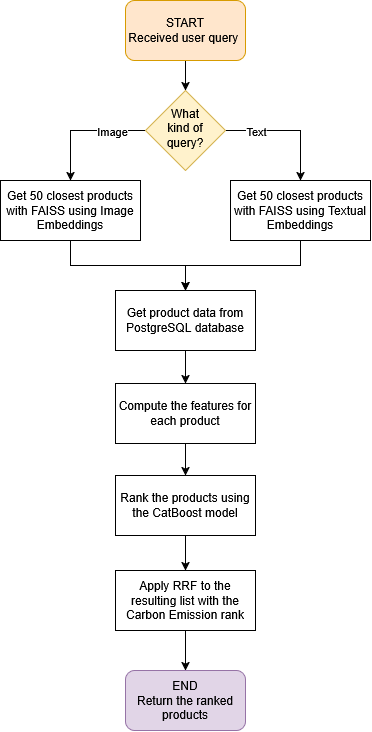
\includegraphics[width=0.85\columnwidth]{fig_ranking_pipeline}}
\caption{Three-stage retrieval and ranking pipeline. A user query (text or image) is embedded via OpenCLIP and matched against the corresponding FAISS index to retrieve the top~50 candidates. Product features are computed from PostgreSQL metadata, re-ranked by CatBoost, and fused with carbon emission rankings through weighted RRF before returning the final ordered list.}
\label{fig:pipeline}
\end{figure}

For text queries, the input is tokenized and encoded via the OpenCLIP text encoder. For image queries, the uploaded image is preprocessed and encoded via the OpenCLIP vision encoder. When both modalities are provided simultaneously, the resulting embeddings are L2-normalized and averaged to produce a fused query vector. The query vector is then matched against the appropriate FAISS index (text or image) to retrieve the top~50 most similar product candidates based on cosine similarity.

\subsection{Hybrid Ranking System}

The 50 candidates retrieved from FAISS are re-ranked using a CatBoost~\cite{catboost} learning-to-rank model, which was selected after careful evaluation of alternatives.

\subsubsection{Model Selection: CatBoost vs. TFRS}

Deep learning frameworks such as TensorFlow Recommenders (TFRS) were initially considered for the ranking engine. However, TFRS fundamentally relies on historical user interaction logs (clicks, purchases, ratings) to learn personalised preferences~\cite{paper1}. Our system is designed as a purely query-driven product search engine: it does not maintain user accounts or track browsing history, and ranking is based entirely on product and platform criteria rather than individual user behaviour. Combined with the project's hardware constraints---a shared server limited to 16\,GB of RAM without a dedicated GPU---a gradient boosting approach proved far more practical. Among boosting algorithms, CatBoost was selected over XGBoost and LightGBM because it requires fewer hyperparameter adjustments and provides built-in mechanisms to reduce overfitting, which is critical when working with small datasets of highly similar electronic products~\cite{catboost}.

\subsubsection{Feature Engineering}

CatBoost re-ranks candidates based on seven engineered features. Prices are normalized using Robust Scaling to mitigate the influence of outlier products (e.g., accessories returned alongside high-value items):
\begin{equation}
z_i = \frac{x_i - \tilde{x}}{Q_3 - Q_1}
\label{eq:robust}
\end{equation}
where $\tilde{x}$ is the median price and $Q_3 - Q_1$ is the interquartile range, followed by min-max normalization to the $[0, 1]$ interval.

Product reliability is computed using a Bayesian weighted average to prevent products with very few reviews from being overvalued:
\begin{equation}
\hat{r}_i = \frac{n_i \cdot \bar{r}_i + C \cdot m}{n_i + C}
\label{eq:bayesian}
\end{equation}
where $n_i$ is the review count, $\bar{r}_i$ is the raw average rating, $C = 5$ is a confidence parameter, and $m = 0.75$ is the prior mean rating.

Since the scraped platforms are direct retailers rather than marketplaces with third-party sellers, no direct seller ratings are available. To approximate seller reliability, we employ three universally available proxy features. The complete set of seven ranking criteria is:

\begin{enumerate}
    \item \textbf{Semantic relevance}: cosine similarity between the query and product embeddings.
    \item \textbf{Price}: robust-scaled and inverted (lower price receives a higher score).
    \item \textbf{Product reliability}: Bayesian weighted average of user ratings (Eq.~\ref{eq:bayesian}).
    \item \textbf{Seller rating}: platform-provided rating when available; defaults to the prior mean $m$ otherwise.
    \item \textbf{Free delivery}: binary indicator serving as a proxy for seller reliability.
    \item \textbf{Return period duration}: robust-scaled number of days; proxy for seller reliability.
    \item \textbf{Warranty duration}: robust-scaled warranty length; proxy for seller reliability.
\end{enumerate}

Additionally, a post-scoring title-matching boost is applied after CatBoost inference. This additive signal rewards products whose names exactly or partially match the user's query, compensating for cases where dense OpenCLIP embeddings---which encode full product descriptions---may dilute brand-name relevance (e.g., returning Samsung devices for an ``iPhone 16'' query).

\subsubsection{Custom Dataset Creation}

No pre-existing dataset was suitable for training the CatBoost model on our specific combination of features. We constructed a custom dataset in LibSVM format through the following process:

\begin{enumerate}
    \item \textbf{Candidate generation}: For each of 40 curated search queries, the FAISS index returned the top 8 most relevant products, yielding approximately 300 initial entries.
    \item \textbf{Negative injection}: A custom negative generator was developed to inject 4 random, out-of-context, or poorly reviewed products per query group, preventing the model from failing to distinguish poor recommendations from relevant ones.
    \item \textbf{LLM-assisted labeling}: Manual relevance labeling (scores 0--3) is historically tedious and resource-intensive. We accelerated dataset creation by utilizing Google Gemini through a few-shot prompting technique, supplying approximately 30 manually labeled examples and strict formatting requirements, enabling the LLM to autonomously label the remaining entries.
    \item \textbf{Data augmentation}: Query groups were duplicated with random row dropping, expanding the dataset to approximately 800 training entries.
\end{enumerate}

\subsubsection{Reciprocal Rank Fusion (RRF)}

Unlike traditional approaches that merge all signals into a single model, our system separates environmental impact from core e-commerce metrics. The CatBoost relevance scores are fused with the carbon footprint estimates using a weighted variant of Reciprocal Rank Fusion~\cite{rrf}:
\begin{equation}
\text{RRF}(d) = \frac{1}{k + r_{\text{rel}}(d)} + w_c \cdot \frac{1}{k + r_{\text{CO}_2}(d)}
\label{eq:rrf}
\end{equation}
where $r_{\text{rel}}(d)$ and $r_{\text{CO}_2}(d)$ are the rank positions of product $d$ in the relevance and carbon rankings respectively, $k = 60$ is the standard RRF damping constant, and $w_c = 0.2$ is the carbon weighting factor. Products without carbon estimates are assigned the last rank position, ensuring they are not penalized but also do not benefit from the carbon signal.

This post-hoc re-ranking mechanism is motivated by recent findings demonstrating that even when absolute carbon estimates are imprecise, ordinal consistency---sorting functionally similar items from greenest to least green---remains highly effective for comparative ranking~\cite{ecommerce_carbon, carbon_reranking}. The system also generates transparent ranking explanations for the top results using the local LLM, promoting environmental awareness during the purchasing process.

\subsection{Carbon Footprint Estimation}

A critical component of the system is evaluating ecological impact despite the absence of formal EPDs in the Vietnamese market. We estimate a Product Carbon Footprint (PCF) based on the cradle-to-grave framework defined by ISO~14067~\cite{iso14067}, encompassing raw material acquisition, manufacturing, distribution, use phase, and end-of-life.

\subsubsection{Carbon Reference Seed Dataset}

To anchor LLM estimates and provide empirical grounding, we curated a reference seed dataset containing products with known or reliably estimated carbon footprint values sourced from published LCA studies and manufacturer EPDs. Each reference product is encoded as a textual OpenCLIP embedding and indexed in a dedicated FAISS inner-product index. For any new product requiring estimation, the system retrieves the $k = 5$ nearest reference products (prioritizing same-category matches) and splits them into \textit{close} neighbours (cosine similarity $\geq 0.66$) and \textit{distant} ones. This threshold was determined empirically: products from the same physical category consistently score above 0.66, while cross-category pairs score below.

\subsubsection{Anchored vs. Unanchored Estimation}

The carbon estimation employs a lightweight, highly quantized Large Language Model (Qwen~3.5 0.8B) served locally via Ollama. This model was selected to minimize computational overhead while maintaining bilingual capability (English and Vietnamese). Estimation follows one of two prompting strategies:

\textbf{Anchored mode} is activated when at least one close neighbour ($\text{sim} \geq 0.66$) exists. The LLM receives the product name, a truncated description, and the close neighbours' known CO\textsubscript{2}e values as calibration anchors. It is instructed to identify the product type, use the references as its primary calibration, and adjust only for clear physical differences. A deviation guard discards any estimate that exceeds a 4$\times$ ratio against the neighbour average.

\textbf{Unanchored mode} is used when no neighbour exceeds the similarity threshold. Instead of potentially misleading cross-category anchors, the LLM receives only the product name, its mapped category label (e.g., ``computer peripheral: mouse, keyboard, webcam''), and the category's known plausibility range as a numeric ballpark. This prevents the model from being anchored to irrelevant reference values.

Both modes use Ollama's structured JSON output enforcement with very low temperature ($T = 0.05$) and a 300-token generation limit, extracting three fields: \texttt{co2e\_kg} (numerical estimate), \texttt{explanation\_en} (one-sentence English explanation), and \texttt{explanation\_vi} (Vietnamese translation).

\subsubsection{Category Bounds and Plausibility Checking}

A critical post-inference validation layer applies category-specific plausibility bounds derived from published manufacturer EPDs, PAIA methodology reports, and IEC~TR~62921 estimates. We define bounds for 41 product categories spanning electronics, home appliances, fashion, beauty, and sports equipment. For example, smartphones are bounded to 10--200\,kg CO\textsubscript{2}e (accommodating foldables), while computer peripherals are bounded to 1--150\,kg. Bounds are intentionally wide to catch only catastrophic hallucinations rather than constraining fine-grained variation.

Additionally, a keyword-based fallback flags small-tech products (speakers, cables, mice, chargers) whose estimates exceed 150\,kg, and global bounds reject values below 0.1\,kg or above 5{,}000\,kg. When the LLM estimate fails any validation check, the system falls back to an unweighted average of the close neighbours' known carbon footprints (if available), assigned a lower confidence score. Products with no close neighbours and a failed LLM estimate are skipped entirely rather than assigned misleading values.

% ================================================================
\section{Preliminary Evaluation}
% ================================================================

\subsection{CatBoost Ranking Performance}

The CatBoost learning-to-rank model was trained on the custom LibSVM dataset of approximately 800 entries derived from 40 search queries. Offline evaluation on a held-out test split yielded a classification accuracy of 95\% on the four-level relevance scale (0--3). While this result is encouraging, we note several caveats: the dataset remains relatively small, and the accuracy metric does not capture nuanced ranking quality measures such as NDCG or MAP, which require a larger and more diverse evaluation corpus with graded relevance annotations.

\subsection{Carbon Estimation Validation}

We evaluate the carbon estimation pipeline using leave-one-out cross-validation on the reference seed dataset. For each of the 30 sampled products, the target is hidden from the index and estimated from the remaining references. Table~\ref{tab:carbon} reports Mean Absolute Error (MAE), Mean Absolute Percentage Error (MAPE), and Spearman rank correlation ($\rho$) for both the neighbour-average baseline and the LLM estimator.

\begin{table}[htbp]
\caption{Carbon estimation: leave-one-out validation ($n=30$)}
\label{tab:carbon}
\centering
\begin{tabular}{lccc}
\toprule
\textbf{Method} & \textbf{MAE (kg)} & \textbf{MAPE (\%)} & \textbf{Spearman} $\rho$ \\
\midrule
Neighbour avg.  & 68.0  & 36.9  & 0.928 \\
LLM (Qwen 3.5 0.8B) & 77.2 & 38.4 & 0.923 \\
\bottomrule
\end{tabular}
\end{table}

Both methods achieve strong ordinal consistency ($\rho > 0.92$), indicating that the system reliably ranks products from lowest to highest carbon footprint within a category. This is the property that matters most for comparative product ranking via RRF.

However, the LLM does not outperform the simpler neighbour-average baseline on any metric. Its absolute errors (MAE~$= 77.2$\,kg, MAPE~$= 38.4\%$) are substantively large. Qualitative analysis reveals that the model performs adequately on well-defined categories where close reference neighbours exist (e.g., smartphones, laptops) but struggles with broader categories such as computer peripherals, where it fails to distinguish between physically dissimilar items. For instance, the model assigned approximately 76\,kg CO\textsubscript{2}e to a standard computer mouse---a product whose actual cradle-to-grave footprint is likely under 5\,kg---because it could not reliably infer the product's physical scale from the Vietnamese-language product name alone.

This finding is consistent with the broader literature. Vestrum et al.~\cite{carbon_reranking} demonstrated that even larger models (Qwen~2.5 3B) exhibit substantial absolute errors (MAE~$= 695$\,kg CO\textsubscript{2}e), though their ordinal rankings remain useful. Spillo et al.~\cite{ecommerce_carbon} showed that frontier models (GPT-o3-mini) achieve strong Spearman correlation ($\rho > 0.96$) despite absolute inaccuracies. Our sub-1B parameter model falls short of these benchmarks, and improving estimation accuracy---particularly for heterogeneous categories---through model scaling, finer-grained category decomposition, or retrieval-augmented generation is a priority for future work.

% ================================================================
\section{Challenges and Limitations}
% ================================================================

\subsection{Processing Speed and Explainability Latency}

Deploying a local LLM introduces significant latency. The two-stage carbon estimation pipeline and the LLM-powered ranking explanation generator both contribute to response times that substantially exceed user expectations for real-time search. This bottleneck is primarily constrained by the lack of GPU hardware on the deployment server.

\subsection{Estimation Accuracy}

As reported in Section~V-B, the 0.8B-parameter model achieves strong ordinal consistency but poor absolute accuracy, particularly for heterogeneous categories. Computer peripherals are a representative failure case: the category spans items from sub-5\,kg mice to 50\,kg+ gaming chairs, yet the model lacks the reasoning depth to reliably infer physical scale from product names. Enabling the model's extended thinking mode did not meaningfully improve estimation precision while substantially increasing inference time and memory consumption---a prohibitive trade-off given the deployment server's resource constraints (16\,GB RAM, no dedicated GPU). The fundamental bottleneck is the model's knowledge representation rather than its inference strategy.

\subsection{Knowledge Cutoff and Data Scarcity}

Because the LLM runs entirely locally and offline, it is limited by its training data cutoff. Newly released products featuring novel eco-friendly materials or manufacturing processes will not be recognized without periodic model updates. Furthermore, the absence of publicly available LCA data and EPDs for electronics in the Vietnamese market prevents robust ground-truth anchoring beyond the curated reference seed dataset.

\subsection{Data Collection Constraints}

Budget limitations prevented the acquisition of commercial proxy infrastructure required to reliably scrape heavily protected marketplace platforms (Shopee, Lazada). Consequently, the system is limited to five specialized electronics retailers, which restricts catalog comprehensiveness. Expanding platform coverage requires either partnerships with retailers or investment in residential proxy networks.

\subsection{Embedding Information Dilution}

Dense OpenCLIP embeddings encode the full product title and description into a single vector, which occasionally causes cross-brand false positives. For example, a query for ``iPhone 16'' may return Samsung devices when their descriptions share technical vocabulary. The post-scoring title-matching boost partially mitigates this issue but represents an ad-hoc solution rather than a principled architectural fix.

% ================================================================
\section{Conclusion and Future Work}
% ================================================================

This paper presented Smart Product Finder, a comprehensive multimodal product recommendation system addressing the dual challenges of price fragmentation and ecological opacity in the Vietnamese e-commerce market. By combining OpenCLIP-powered multimodal search, CatBoost learning-to-rank, and Reciprocal Rank Fusion with LLM-estimated carbon footprints, the system provides users with optimized and environmentally informed purchasing recommendations across five major Vietnamese retailers.

The current implementation demonstrates the viability of the architectural approach, with the CatBoost ranking model achieving promising offline performance and the RRF fusion mechanism successfully integrating environmental signals. However, the carbon estimation component requires further refinement, particularly through model scaling or retrieval-augmented generation techniques.

Future work will focus on four key directions: (1)~upgrading to larger language models with improved reasoning capabilities, supported by better server infrastructure including GPU acceleration; (2)~integrating retrieval-augmented generation (RAG) to bypass knowledge cutoffs by dynamically incorporating up-to-date LCA data and manufacturer sustainability reports; (3)~exploring cost-effective data aggregation strategies, including retailer API partnerships, to expand platform coverage; and (4)~expanding the evaluation corpus with a larger, more diverse set of annotated queries to enable reporting of standard information retrieval metrics such as NDCG and MAP.

% ================================================================
% REFERENCES
% ================================================================
\begin{thebibliography}{00}

\bibitem{paper1}
S.~Tulasi~T and I.~Ahamed~S~B, ``AI-powered e-commerce personalization and recommendation systems,'' \textit{J. Informatics Educ. Res.}, vol.~5, no.~1, pp.~2092--2099, 2025.

\bibitem{paper2}
B.~R.~V.~Naga~Chandra~Reddy \textit{et~al.}, ``AI-powered e-commerce platform for small businesses,'' \textit{Int. J. Innov. Sci. Res. Technol.}, vol.~10, no.~4, pp.~495--501, Apr. 2025.

\bibitem{paper3}
M.~Raj, V.~Saroj, S.~Sen, Y.~Mittal, S.~Gupta, and A.~Shukla, ``AI-powered price comparison for e-commerce food rides,'' in \textit{Proc. 7th Int. Conf. Inf. Syst. Comput. Netw. (ISCON)}, Mathura, India, 2025.

\bibitem{paper4}
A.~Jayaraj, P.~Nair, S.~T~R, A.~Raj, A.~R, and G.~B~Shankar, ``Intelligent market insight: A multi-agent system for artificial intelligence powered shopping optimization,'' in \textit{Proc. 3rd Int. Conf. Sustain. Comput. Data Commun. Syst. (ICSCDS)}, 2025.

\bibitem{paper5}
B.~Zhang, Y.~Han, and X.~Han, ``Research on multi-modal retrieval system of e-commerce platform based on pre-training model,'' \textit{Artif. Intell. Technol. Res.}, vol.~2, no.~9, pp.~86--89, 2025.

\bibitem{carbon_reranking}
A.~Vestrum, J.~Bergh, and N.~L.~Syrdal, ``Trading engagement for sustainability: Carbon-aware re-ranking for e-commerce recommendations,'' \textit{arXiv preprint arXiv:2606.04550}, 2026.

\bibitem{carbon_estimation}
F.~Xu, D.~Xiang, K.~Fang, and G.~Chen, ``Carbon footprint estimation and carbon data validation in the manufacturing phase of electromechanical products,'' \textit{Chin. J. Mech. Eng.}, vol.~39, art.~100157, 2026.

\bibitem{ecommerce_carbon}
G.~Spillo, A.~De~Filippo, C.~Musto, M.~Milano, and G.~Semeraro, ``Eco-Amazon: Enriching e-commerce datasets with product carbon footprint for sustainable recommendations,'' \textit{arXiv preprint arXiv:2602.15508}, 2026.

\bibitem{catboost}
L.~Prokhorenkova, G.~Gusev, A.~Vorobev, A.~V.~Dorogush, and A.~Gulin, ``CatBoost: Unbiased boosting with categorical features,'' in \textit{Advances in Neural Information Processing Systems (NeurIPS)}, 2018, pp.~6638--6648.

\bibitem{openclip}
M.~Cherti, R.~Beaumont, R.~Wightman, M.~Wortsman, G.~Ilharco, C.~Gordon, C.~Schuhmann, L.~Schmidt, and J.~Jitsev, ``Reproducible scaling laws for contrastive language--image learning,'' in \textit{Proc. IEEE/CVF Conf. Comput. Vis. Pattern Recognit. (CVPR)}, 2023, pp.~2818--2829.

\bibitem{faiss}
J.~Johnson, M.~Douze, and H.~J\'egou, ``Billion-scale similarity search with GPUs,'' \textit{IEEE Trans. Big Data}, vol.~7, no.~3, pp.~535--547, 2021.

\bibitem{rrf}
G.~V.~Cormack, C.~L.~A.~Clarke, and S.~B\"uttcher, ``Reciprocal rank fusion outperforms condorcet and individual rank learning methods,'' in \textit{Proc. 32nd Int. ACM SIGIR Conf. Res. Develop. Inf. Retrieval}, 2009, pp.~758--759.

\bibitem{iso14067}
ISO~14067:2018, ``Greenhouse gases---Carbon footprint of products---Requirements and guidelines for quantification,'' International Organization for Standardization, Geneva, Switzerland, 2018.

\end{thebibliography}

\end{document}
